 \documentclass[oneside,11pt]{article}

\input{preamble.tex}
%%% HELPER CODE FOR DEALING WITH EXTERNAL REFERENCES
\usepackage{xr}
\makeatletter
\newcommand*{\addFileDependency}[1]{
  \typeout{(#1)}
  \@addtofilelist{#1}
  \IfFileExists{#1}{}{\typeout{No file #1.}}
}
\makeatother


\newcommand*{\myexternaldocument}[1]{
    \externaldocument{#1}
    \addFileDependency{#1.tex}
    \addFileDependency{#1.aux}
}

%\myexternaldocument{OA}

%%%%%%%%%%%%%%%%%%%%%%%%%%%%%%%% DOCUMENT
\begin{document}


\title{Bargaining with (more) common priors in the field \thanks{We want to thank}}
\author{Joyce Sadka \and Enrique Seira  \and Christopher Woodruff \thanks{\protect\linespread{1}\protect\selectfont Sadka: ITAM, jsadka@itam.mx;  
Seira: ITAM, enrique.seira@itam.mx; Woodruff (corresponding author): University of Oxford, Department of International Development, Oxford OX13TB, UK, christopher.woodruff@qeh.ox.ac.uk.} }
\date{This draft:  \today \\[2 cm]}

%\vspace{.5in}


\maketitle
\thispagestyle{empty}
\begin{abstract}

Several theoretical models have shown that bargaining can break down if parties have different priors about the probability of winning at trial. We test this theory in the field by studying labor conflicts. First, we run an experiment providing information about likely outcomes at trial to a treatment group that includes both plaintiff and defendants.  We show that they update expectations in the direction of the information and it makes it closer to the employers expectation, and that they settle more compared to a control group. Second, we show that providing information to only the worker has much smaller effects. Third, we exploit a discontinuity in the information provision rule and show that (otherwise identical) parties that get information with a higher predicted payment to the worker update their priors upward (and come closer together) and settle more, consistent with bargaining models of bargaining with common priors (or models increasing the bargaining power of the weakest player XXX) decreases bargaining impasses. Finally, we show that providing predictive information that is too far off from their own priors makes them update expectations less, and lowers the effect of the information on settlement rates. This suggests that they have private information on their own case and disregard information that is less consistent with their information. All in all we show that information provided to both parties increases settlement more.


\end{abstract}

\vspace{.3in}

\textbf{Keywords: } 

\textbf{JEL codes:} G41, C93, O16, G21

\newpage

\pagenumbering{arabic}
\etocdepthtag.toc{mtchapter}
\etocsettagdepth{mtchapter}{subsection}
\etocsettagdepth{mtappendix}{none}



\section{Introduction}

[CW: There are interesting results for the Letter, but they are quite different from the Calculator. The Calculator treatment is clearer - we gave information to one party, so both empowered and incentivized the worker to settle above the threshold. In the Letter treatment, we empowered both parties equally (and hence, neither of them) and the incentives are zero-sum.] \\




We examine outcomes of bargaining between employees claiming severance payment and their previous employers who are liable for any payments. We provide parties with estimated values of the claims derived from a coarse prediction model that partitions 400 workers into four quadrants based on their wage and tenure at the firm. The model is based on 5000 outcomes of past cases in the Mexico City Labor Court.  We exploit the sharp discontinuities in the expected value of the employees claims, identifying workers with very similar wages and tenures, but who fall on either side of cutoffs associated a large change in the expected value of the claim and identifying workers at either edge of a given partition who are therefore provided with the same prediction but who circumstances different. We find that workers with similar characteristics who are provided with higher valuations are more likely to reach a settlement with their employers and reach larger settlements when they do settle. Workers who are at the top end of the partitions - those for whom a finer model would predict higher outcomes - are less likely to settle, suggesting that they understand that the valuation provided is too low. Both of these results suggest that the workers’ expectations drive the bargaining process, perhaps because the institutions governing the bargaining process function more poorly than workers believe. 

What do we learn from this? 
\begin{itemize}
    \item Information affects the probability of settlement, and the amount conditional on settlement. (This seems to say that workers are the constraint here. Probably that is because the court works much worse for workers than they expect, so they lower valuations are too far from what they expect. But we don't know if maybe the amounts are too low for all of the workers, even including those receiving the higher valuations.)
    \item Workers are sophisticated enough to know that the prediction is too low, or get advice that indicates that to them.
\end{itemize}




\newpage
%%%%%%%%%%%%%%%%%%%%%%%%%%%%%%%%%%%%%%%%%%%%%%%%%%%%%%%%%%%%%
%BIBLIOGRAPHY


\clearpage
\bibliographystyle{authordate1}
%\bibliographystyle{amsalpha}
%\bibliographystyle{AER}

\bibliography{References}



%\FloatBarrier
%%%%%%%%%%%%%%%%%%%%%%%%%%%%%%%%%%%%%%%%

\newpage
\singlespacing



\begin{figure}[H]
     \caption{RD design}
    \label{rd_design}
\begin{center}
\begin{subfigure}{0.75\textwidth}
        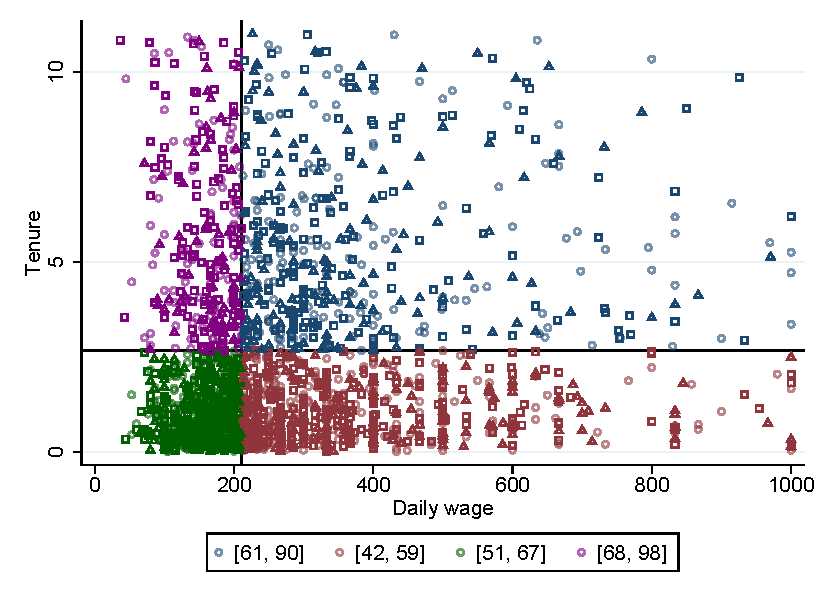
\includegraphics[width=\textwidth]{Figuras/scatter_rddesign.pdf}
    \end{subfigure}
  \end{center}
    \scriptsize 
%\textit{Scripts: }  \texttt{scatter\_runningvars.do}
\end{figure}


\begin{figure}[H]
     \caption{Manipulation test}
    \label{manipulation_test}
\begin{center}
\begin{subfigure}{0.49\textwidth}
\caption{Tenure}
        \includegraphics[width=\textwidth]{Figuras/mtp_tenure.pdf}
    \end{subfigure}
    \begin{subfigure}{0.49\textwidth}
\caption{Daily wage}
        \includegraphics[width=\textwidth]{Figuras/mtp_dw.pdf}
    \end{subfigure}
\begin{subfigure}{0.49\textwidth}
\caption{Tenure \& Daily wage}
        \includegraphics[width=\textwidth]{Figuras/mtp_index.pdf}
    \end{subfigure}
  \end{center}
  
    \scriptsize Manipulation testing based on density continuity.
%\textit{Scripts: }  \texttt{manipulation\_tests.do}
\end{figure}




\begin{landscape}
\begin{table}[H]
\caption{Balance table (Calculator treatment)}
\label{balance_table_t2_tenure}
\begin{center}
\resizebox{1.5\textwidth}{!}{
\scriptsize{% Table generated by Excel2LaTeX from sheet 'rd_balance_t2'
\begin{tabular}{lcccccccccc}
\toprule
      & \multicolumn{10}{c}{Running variable: Tenure} \\
\midrule
      & Anger & + High-school & Recruitment & At will  & Weekly hours & Inf. worker & Legal ent. & Total ent. & Top sued & Women \\
\midrule
      & (1)   & (2)   & (3)   & (4)   & (5)   & (6)   & (7)   & (8)   & (9)   & (10) \\
\midrule
\midrule
Conventional & 0.504 & 0.101 & 0.223 & -0.0140 & -1.293 & -0.0333 & 1,718 & 2,504 & -0.0778 & -0.0358 \\
      & (0.698) & (0.162) & (0.197) & (0.0806) & (4.783) & (0.133) & (5,326) & (6,373) & (0.0817) & (0.173) \\
Robust & 0.596 & 0.0859 & 0.290 & -0.00519 & -2.325 & -0.0476 & 478.7 & 1,206 & -0.0890 & -0.0220 \\
      & (0.815) & (0.193) & (0.222) & (0.0909) & (5.572) & (0.152) & (6,168) & (7,383) & (0.0926) & (0.201) \\
      &       &       &       &       &       &       &       &       &       &  \\
\midrule
Control Mean & 8.146 & 0.730 & 0.253 & 0.0544 & 52.76 & 0.255 & 25157 & 30476 & 0.0460 & 0.488 \\
Effective observations [L , R] & [97 , 53] & [119 , 63] & [66 , 42] & [111 , 62] & [67 , 42] & [105 , 58] & [101 , 57] & [101 , 57] & [101 , 57] & [127 , 65] \\
Bandwidth [L , R] & [0.977 , 0.977] & [1.167 , 1.167] & [0.689 , 0.689] & [1.098 , 1.098] & [0.698 , 0.698] & [1.002 , 1.002] & [0.966 , 0.966] & [0.970 , 0.970] & [0.981 , 0.981] & [1.210 , 1.210] \\
\midrule
\midrule
      &       &       &       &       &       &       &       &       &       &  \\
\midrule
      & \multicolumn{10}{c}{Running variable: Daily wage} \\
\midrule
      & Anger & + High-school & Recruitment & At will  & Weekly hours & Inf. worker & Legal ent. & Total ent. & Top sued & Women \\
\midrule
      & (11)  & (12)  & (13)  & (14)  & (15)  & (16)  & (17)  & (18)  & (19)  & (20) \\
\midrule
\midrule
Conventional & 0.615 & -0.232** & 0.000805 & -0.0529 & 1.683 & -0.106 & -2.14e-05 & -2,510 & -0.0372 & -0.294** \\
      & (0.447) & (0.117) & (0.0958) & (0.0363) & (3.409) & (0.0993) & (14.21) & (1,858) & (0.0746) & (0.148) \\
Robust & 0.788 & -0.239* & 0.0448 & -0.0653* & 0.779 & -0.0977 & 1.75e-05 & -3,342 & -0.0647 & -0.393** \\
      & (0.539) & (0.142) & (0.114) & (0.0361) & (4.172) & (0.121) & (17.96) & (2,267) & (0.0915) & (0.176) \\
      &       &       &       &       &       &       &       &       &       &  \\
\midrule
Control Mean & 8.033 & 0.596 & 0.173 & 0.0440 & 51.17 & 0.286 & 14207 & 21411 & 0.0660 & 0.522 \\
Effective observations [L , R] & [158 , 115] & [173 , 121] & [135 , 109] & [167 , 118] & [168 , 118] & [175 , 122] & [132 , 109] & [114 , 99] & [174 , 120] & [99 , 89] \\
Bandwidth [L , R] & [49.69 , 49.69] & [52.12 , 52.12] & [41 , 41] & [47.57 , 47.57] & [48.14 , 48.14] & [52.44 , 52.44] & [39.65 , 39.65] & [34.25 , 34.25] & [51.49 , 51.49] & [28.67 , 28.67] \\
\midrule
\midrule
      &       &       &       &       &       &       &       &       &       &  \\
\midrule
      & \multicolumn{10}{c}{Running variable: Tenure \& Daily wage} \\
\midrule
      & Anger & + High-school & Recruitment & At will  & Weekly hours & Inf. worker & Legal ent. & Total ent. & Top sued & Women \\
\midrule
      & (21)  & (22)  & (23)  & (24)  & (25)  & (26)  & (27)  & (28)  & (29)  & (30) \\
\midrule
\midrule
Conventional & 0.812 & 0.0886 & 0.0391 & -0.191 & 5.046 & -0.0369 & -1,341 & -2,917* & -0.0323 & 0.199 \\
      & (0.845) & (0.216) & (0.153) & (0.148) & (6.310) & (0.170) & (1,141) & (1,706) & (0.189) & (0.215) \\
Robust & 1.029 & 0.111 & 0.0728 & -0.232 & 6.441 & -0.0501 & -1,449 & -3,288* & -0.0830 & 0.260 \\
      & (1.018) & (0.261) & (0.185) & (0.174) & (7.805) & (0.205) & (1,279) & (1,907) & (0.233) & (0.259) \\
      &       &       &       &       &       &       &       &       &       &  \\
\midrule
Control Mean & 8.132 & 0.804 & 0.296 & 0.0846 & 53.72 & 0.212 & 34261 & 41028 & 0.0346 & 0.425 \\
Effective observations [L , R] & [187 , 53] & [200 , 59] & [203 , 62] & [93 , 33] & [170 , 52] & [187 , 55] & [30 , 24] & [40 , 26] & [164 , 50] & [181 , 55] \\
Bandwidth [L , R] & [0.961 , 0.961] & [1.017 , 1.017] & [1.098 , 1.098] & [0.499 , 0.499] & [0.756 , 0.756] & [0.880 , 0.880] & [0.330 , 0.330] & [0.356 , 0.356] & [0.721 , 0.721] & [0.838 , 0.838] \\
\bottomrule
\bottomrule
\end{tabular}%
}
}
\end{center}
 \scriptsize 
\textit{Do file: } \texttt{balance\_table.do}
\end{table}


\begin{table}[H]
\caption{Balance table (Calculator + letter treatment)}
\label{balance_table_t2_tenure}
\begin{center}
\resizebox{1.5\textwidth}{!}{
\scriptsize{% Table generated by Excel2LaTeX from sheet 'rd_balance_t3'
\begin{tabular}{lcccccccccc}
\toprule
      & \multicolumn{10}{c}{Running variable: Tenure} \\
\midrule
      & Anger & + High-school & Recruitment & At will  & Weekly hours & Inf. worker & Legal ent. & Total ent. & Top sued & Women \\
\midrule
      & (1)   & (2)   & (3)   & (4)   & (5)   & (6)   & (7)   & (8)   & (9)   & (10) \\
\midrule
\midrule
Conventional & -1.132 & -0.0550 & -0.928*** & -0.184 & -5.385 & 0.177 & -13,555 & -12,500 & 0     & 0.253 \\
      & (1.180) & (0.213) & (0.352) & (0.338) & (10.21) & (0.204) & (11,774) & (13,351) & (0.000567) & (0.226) \\
Robust & -1.410 & -0.0876 & -1.028*** & -0.212 & -4.568 & 0.202 & -16,120 & -15,058 & -0.00739 & 0.289 \\
      & (1.362) & (0.251) & (0.382) & (0.377) & (12.32) & (0.241) & (13,174) & (15,125) & (0.00754) & (0.265) \\
      &       &       &       &       &       &       &       &       &       &  \\
\midrule
Control Mean & 8.319 & 0.717 & 0.249 & 0.0308 & 54.74 & 0.274 & 25444 & 30464 & 0.0492 & 0.477 \\
Effective observations [L , R] & [62 , 43] & [67 , 53] & [17 , 17] & [26 , 27] & [27 , 27] & [45 , 38] & [29 , 27] & [34 , 34] & [43 , 37] & [57 , 43] \\
Bandwidth [L , R] & [1.043 , 1.043] & [1.142 , 1.142] & [0.471 , 0.471] & [0.631 , 0.631] & [0.668 , 0.668] & [0.822 , 0.822] & [0.694 , 0.694] & [0.743 , 0.743] & [0.809 , 0.809] & [1 , 1] \\
\midrule
\midrule
      &       &       &       &       &       &       &       &       &       &  \\
\midrule
      & \multicolumn{10}{c}{Running variable: Daily wage} \\
\midrule
      & Anger & + High-school & Recruitment & At will  & Weekly hours & Inf. worker & Legal ent. & Total ent. & Top sued & Women \\
\midrule
      & (11)  & (12)  & (13)  & (14)  & (15)  & (16)  & (17)  & (18)  & (19)  & (20) \\
\midrule
\midrule
Conventional & -0.162 & 0.0764 & 0.0368 & -0.0207 & 3.280 & -0.00335 & -0.000164 & -2,857 & -0.00796 & 0.204 \\
      & (0.654) & (0.142) & (0.124) & (0.0236) & (4.904) & (0.174) & (27.37) & (2,336) & (0.0493) & (0.129) \\
Robust & -0.249 & 0.0887 & 0.0135 & -0.0254 & 5.315 & -0.0613 & -0.000211 & -3,680 & -0.0292 & 0.232 \\
      & (0.809) & (0.178) & (0.155) & (0.0253) & (5.879) & (0.215) & (34.69) & (2,829) & (0.0586) & (0.157) \\
      &       &       &       &       &       &       &       &       &       &  \\
\midrule
Control Mean & 8.255 & 0.583 & 0.202 & 0.0219 & 50.93 & 0.259 & 14242 & 21015 & 0.0526 & 0.553 \\
Effective observations [L , R] & [113 , 74] & [143 , 92] & [140 , 92] & [100 , 67] & [143 , 92] & [117 , 67] & [100 , 67] & [100 , 67] & [144 , 93] & [160 , 95] \\
Bandwidth [L , R] & [48.13 , 48.13] & [58.88 , 58.88] & [57.13 , 57.13] & [43.17 , 43.17] & [58.66 , 58.66] & [45.30 , 45.30] & [41.80 , 41.80] & [41.83 , 41.83] & [60.20 , 60.20] & [66.11 , 66.11] \\
\midrule
\midrule
      &       &       &       &       &       &       &       &       &       &  \\
\midrule
      & \multicolumn{10}{c}{Running variable: Tenure \& Daily wage} \\
\midrule
      & Anger & + High-school & Recruitment & At will  & Weekly hours & Inf. worker & Legal ent. & Total ent. & Top sued & Women \\
\midrule
      & (21)  & (22)  & (23)  & (24)  & (25)  & (26)  & (27)  & (28)  & (29)  & (30) \\
\midrule
\midrule
Conventional & -0.146 & -0.123 & 0.0351 & 0     & 10.60 & -0.274 & 1,649 & 2,950 & 0.0463 & -0.0512 \\
      & (1.150) & (0.321) & (0.353) & (0)   & (14.83) & (0.307) & (3,858) & (4,362) & (0.0533) & (0.301) \\
Robust & -0.288 & -0.132 & 0.128 & -0.0225 & 16.23 & -0.232 & 987.5 & 1,823 & 0.0477 & -0.0692 \\
      & (1.438) & (0.402) & (0.437) & (0.0223) & (18.16) & (0.373) & (4,233) & (5,003) & (0.0659) & (0.371) \\
      &       &       &       &       &       &       &       &       &       &  \\
\midrule
Control Mean & 8.308 & 0.811 & 0.268 & 0.0610 & 57.84 & 0.256 & 36500 & 43367 & 0.0549 & 0.421 \\
Effective observations [L , R] & [76 , 29] & [86 , 37] & [75 , 32] & [6 , 12] & [60 , 29] & [38 , 23] & [11 , 15] & [21 , 16] & [22 , 17] & [91 , 38] \\
Bandwidth [L , R] & [0.638 , 0.638] & [0.713 , 0.713] & [0.620 , 0.620] & [0.244 , 0.244] & [0.529 , 0.529] & [0.474 , 0.474] & [0.297 , 0.297] & [0.345 , 0.345] & [0.353 , 0.353] & [0.770 , 0.770] \\
\bottomrule
\bottomrule
\end{tabular}%
}
}
\end{center}
 \scriptsize 
\textit{Do file: } \texttt{balance\_table.do}
\end{table}


\end{landscape}

%__________________________________________________________________________
%__________________________________________________________________________
%__________________________________________________________________________
%__________________________________________________________________________

\clearpage

\begin{landscape}
\begin{table}[H]
\caption{Regression discontinuity - Effect on solved conflict}
\label{rd_sett}
\begin{center}
\scriptsize{% Table generated by Excel2LaTeX from sheet 'rd_sett'
\begin{tabular}{lcccccccc}
\toprule
      & \multicolumn{8}{c}{Calculator treatment} \\
\midrule
      & \multicolumn{2}{c}{Tenure} &       & \multicolumn{2}{c}{Daily wage} &       & \multicolumn{2}{c}{Tenure \& Daily wage} \\
\cmidrule{2-3}\cmidrule{5-6}\cmidrule{8-9}      & (1)   & (2)   &       & (3)   & (4)   &       & (5)   & (6) \\
\midrule
\midrule
Conventional & 0.397** & 0.391*** &       & -0.179 & -0.214 &       & 0.338 & 0.421** \\
      & (0.158) & (0.150) &       & (0.127) & (627.5) &       & (0.225) & (0.197) \\
Robust & 0.420** & 0.390** &       & -0.231 & -0.262 &       & 0.385 & 0.476* \\
      & (0.183) & (0.174) &       & (0.152) & (805.6) &       & (0.275) & (0.243) \\
      &       &       &       &       &       &       &       &  \\
\midrule
Effective observations [L , R] & [109 ,  61] & [104 ,  56] &       & [137 ,  111] & [125 ,  106] &       & [146 ,  44] & [139 ,  42] \\
Bandwidth [L , R] & [1.067 ,  1.067] & [1.067 ,  1.067] &       & [42.28 ,  42.28] & [42.28 ,  42.28] &       & [0.634 ,  0.634] & [0.634 ,  0.634] \\
Controls &       & \checkmark &       &       & \checkmark &       &       & \checkmark \\
\midrule
\midrule
      &       &       &       &       &       &       &       &  \\
      &       &       &       &       &       &       &       &  \\
\midrule
      & \multicolumn{8}{c}{Calculator + letter treatment} \\
\midrule
      & \multicolumn{2}{c}{Tenure} &       & \multicolumn{2}{c}{Daily wage} &       & \multicolumn{2}{c}{Tenure \& Daily wage} \\
\cmidrule{2-3}\cmidrule{5-6}\cmidrule{8-9}      & (1)   & (2)   &       & (3)   & (4)   &       & (5)   & (6) \\
\midrule
\midrule
Conventional & -0.367** & -0.354** &       & 0.0645 & 0.0570 &       & 0.223 & 0.265 \\
      & (0.179) & (0.170) &       & (0.121) & (0.109) &       & (0.289) & (0.281) \\
Robust & -0.430** & -0.404** &       & 0.0731 & 0.0507 &       & 0.216 & 0.251 \\
      & (0.199) & (0.193) &       & (0.148) & (0.136) &       & (0.357) & (0.351) \\
      &       &       &       &       &       &       &       &  \\
\midrule
Effective observations [L , R] & [58 ,  44] & [56 ,  41] &       & [160 ,  95] & [153 ,  93] &       & [97 ,  38] & [95 ,  35] \\
Bandwidth [L , R] & [1.008 ,  1.008] & [1.008 ,  1.008] &       & [65.75 ,  65.75] & [65.75 ,  65.75] &       & [0.821 ,  0.821] & [0.821 ,  0.821] \\
Controls &       & \checkmark &       &       & \checkmark &       &       & \checkmark \\
\bottomrule
\bottomrule
\end{tabular}%
}
\end{center}
\scriptsize{
Table reports the RD coefficients obtained for the discontinuities in the calculator prediction. Columns (1) and (2) report the coefficients for the discontinuity along the tenure dimension. Columns (3) and (4) report the coefficients for the discontinuity along the wage dimension. Columns (5) and (6) report the coefficients for the discontinuity along both tenure and wage dimensions, taking the euclidean distance from the join cutoff. The upper panel reports the coefficients for the calculator treatment arm. The lower panel reports the coefficients for the calculator + letter treatment arm. Conventional RD coefficients report the estimates with conventional variance estimator. Robust RD coefficients report the bias-corrected estimates with robust variance estimator.}

 \scriptsize 
\textit{Do file: } \texttt{rd\_results.do}
\end{table}
\end{landscape}

\clearpage

\begin{landscape}
\begin{table}[H]
\caption{Regression discontinuity - Effect on suing}
\label{rd_sued}
\begin{center}
\scriptsize{% Table generated by Excel2LaTeX from sheet 'rd_sued'
\begin{tabular}{lcccccccc}
\toprule
      & \multicolumn{8}{c}{Calculator treatment} \\
\midrule
      & \multicolumn{2}{c}{Tenure} &       & \multicolumn{2}{c}{Daily wage} &       & \multicolumn{2}{c}{Tenure \& Daily wage} \\
\cmidrule{2-3}\cmidrule{5-6}\cmidrule{8-9}      & (1)   & (2)   &       & (3)   & (4)   &       & (5)   & (6) \\
\midrule
\midrule
Conventional & -0.251 & -0.260 &       & 0.0990 & 0.136 &       & -0.351* & -0.444** \\
      & (0.161) & (0.158) &       & (0.103) & (0.104) &       & (0.213) & (0.175) \\
Robust & -0.288 & -0.289 &       & 0.107 & 0.135 &       & -0.425* & -0.516** \\
      & (0.187) & (0.184) &       & (0.125) & (0.127) &       & (0.252) & (0.208) \\
      &       &       &       &       &       &       &       &  \\
\midrule
Effective observations [L , R] & [128 ,  65] & [126 ,  62] &       & [225 ,  155] & [218 ,  154] &       & [143 ,  45] & [140 ,  44] \\
Bandwidth [L , R] & [1.228 ,  1.228] & [1.228 ,  1.228] &       & [72.11 ,  72.11] & [72.11 ,  72.11] &       & [0.642 ,  0.642] & [0.642 ,  0.642] \\
Controls &       & \checkmark &       &       & \checkmark &       &       & \checkmark \\
\midrule
\midrule
      &       &       &       &       &       &       &       &  \\
      &       &       &       &       &       &       &       &  \\
\midrule
      & \multicolumn{8}{c}{Calculator + letter treatment} \\
\midrule
      & \multicolumn{2}{c}{Tenure} &       & \multicolumn{2}{c}{Daily wage} &       & \multicolumn{2}{c}{Tenure \& Daily wage} \\
\cmidrule{2-3}\cmidrule{5-6}\cmidrule{8-9}      & (1)   & (2)   &       & (3)   & (4)   &       & (5)   & (6) \\
\midrule
\midrule
Conventional & -0.0229 & 0.0200 &       & -0.0342 & -0.0446 &       & -0.353 & -0.354 \\
      & (0.297) & (0.252) &       & (0.157) & (0.144) &       & (0.364) & (0.318) \\
Robust & -0.0359 & 0.0458 &       & -0.0341 & -0.0327 &       & -0.440 & -0.418 \\
      & (0.352) & (0.301) &       & (0.200) & (0.185) &       & (0.450) & (0.392) \\
      &       &       &       &       &       &       &       &  \\
\midrule
Effective observations [L , R] & [44 ,  35] & [44 ,  35] &       & [134 ,  78] & [133 ,  78] &       & [76 ,  29] & [76 ,  29] \\
Bandwidth [L , R] & [0.822 ,  0.822] & [0.822 ,  0.822] &       & [55.01 ,  55.01] & [55.01 ,  55.01] &       & [0.641 ,  0.641] & [0.641 ,  0.641] \\
Controls &       & \checkmark &       &       & \checkmark &       &       & \checkmark \\
\bottomrule
\bottomrule
\end{tabular}%
}
\end{center}
\scriptsize{
Table reports the RD coefficients obtained for the discontinuities in the calculator prediction. Columns (1) and (2) report the coefficients for the discontinuity along the tenure dimension. Columns (3) and (4) report the coefficients for the discontinuity along the wage dimension. Columns (5) and (6) report the coefficients for the discontinuity along both tenure and wage dimensions, taking the euclidean distance from the join cutoff. The upper panel reports the coefficients for the calculator treatment arm. The lower panel reports the coefficients for the calculator + letter treatment arm. Conventional RD coefficients report the estimates with conventional variance estimator. Robust RD coefficients report the bias-corrected estimates with robust variance estimator.}

 \scriptsize 
\textit{Do file: } \texttt{rd\_results.do}
\end{table}
\end{landscape}

\clearpage

\begin{landscape}
\begin{table}[H]
\caption{Regression discontinuity - Effect on suing with a public lawyer}
\label{rd_sued_public}
\begin{center}
\scriptsize{% Table generated by Excel2LaTeX from sheet 'rd_sued_public'
\begin{tabular}{lcccccccc}
\toprule
      & \multicolumn{8}{c}{Calculator treatment} \\
\midrule
      & \multicolumn{2}{c}{Tenure} &       & \multicolumn{2}{c}{Daily wage} &       & \multicolumn{2}{c}{Tenure \& Daily wage} \\
\cmidrule{2-3}\cmidrule{5-6}\cmidrule{8-9}      & (1)   & (2)   &       & (3)   & (4)   &       & (5)   & (6) \\
\midrule
\midrule
Conventional & -0.155 & -0.162 &       & -0.00695 & 0.00366 &       & -0.0638 & -0.158 \\
      & (0.117) & (0.111) &       & (0.0845) & (0.0841) &       & (0.149) & (0.118) \\
Robust & -0.158 & -0.153 &       & -0.0278 & -0.0260 &       & -0.0924 & -0.194 \\
      & (0.138) & (0.131) &       & (0.103) & (0.102) &       & (0.178) & (0.145) \\
      &       &       &       &       &       &       &       &  \\
\midrule
Effective observations [L , R] & [110 ,  61] & [109 ,  58] &       & [169 ,  118] & [163 ,  117] &       & [188 ,  54] & [183 ,  51] \\
Bandwidth [L , R] & [1.131 ,  1.131] & [1.131 ,  1.131] &       & [53.48 ,  53.48] & [53.48 ,  53.48] &       & [0.921 ,  0.921] & [0.921 ,  0.921] \\
Controls &       & \checkmark &       &       & \checkmark &       &       & \checkmark \\
\midrule
\midrule
      &       &       &       &       &       &       &       &  \\
      &       &       &       &       &       &       &       &  \\
\midrule
      & \multicolumn{8}{c}{Calculator + letter treatment} \\
\midrule
      & \multicolumn{2}{c}{Tenure} &       & \multicolumn{2}{c}{Daily wage} &       & \multicolumn{2}{c}{Tenure \& Daily wage} \\
\cmidrule{2-3}\cmidrule{5-6}\cmidrule{8-9}      & (1)   & (2)   &       & (3)   & (4)   &       & (5)   & (6) \\
\midrule
\midrule
Conventional & -0.395 & -0.202 &       & -0.120 & -0.134 &       & -0.0995 & -0.0707 \\
      & (0.294) & (0.211) &       & (0.104) & (0.103) &       & (0.280) & (0.250) \\
Robust & -0.423 & -0.183 &       & -0.133 & -0.147 &       & -0.127 & -0.0783 \\
      & (0.336) & (0.240) &       & (0.130) & (0.127) &       & (0.350) & (0.312) \\
      &       &       &       &       &       &       &       &  \\
\midrule
Effective observations [L , R] & [34 ,  29] & [34 ,  29] &       & [153 ,  93] & [152 ,  93] &       & [80 ,  32] & [80 ,  32] \\
Bandwidth [L , R] & [0.714 ,  0.714] & [0.714 ,  0.714] &       & [64.83 ,  64.83] & [64.83 ,  64.83] &       & [0.651 ,  0.651] & [0.651 ,  0.651] \\
Controls &       & \checkmark &       &       & \checkmark &       &       & \checkmark \\
\bottomrule
\bottomrule
\end{tabular}%
}
\end{center}
\scriptsize{
Table reports the RD coefficients obtained for the discontinuities in the calculator prediction. Columns (1) and (2) report the coefficients for the discontinuity along the tenure dimension. Columns (3) and (4) report the coefficients for the discontinuity along the wage dimension. Columns (5) and (6) report the coefficients for the discontinuity along both tenure and wage dimensions, taking the euclidean distance from the join cutoff. The upper panel reports the coefficients for the calculator treatment arm. The lower panel reports the coefficients for the calculator + letter treatment arm. Conventional RD coefficients report the estimates with conventional variance estimator. Robust RD coefficients report the bias-corrected estimates with robust variance estimator.}

 \scriptsize 
\textit{Do file: } \texttt{rd\_results.do}
\end{table}
\end{landscape}

\clearpage

\begin{figure}[H]
     \caption{RD plots (Calculator treatment) - Effect on solved conflict}
    \label{rd_t2}
\begin{center}
\begin{subfigure}{0.31\textwidth}

\caption{Tenure}
        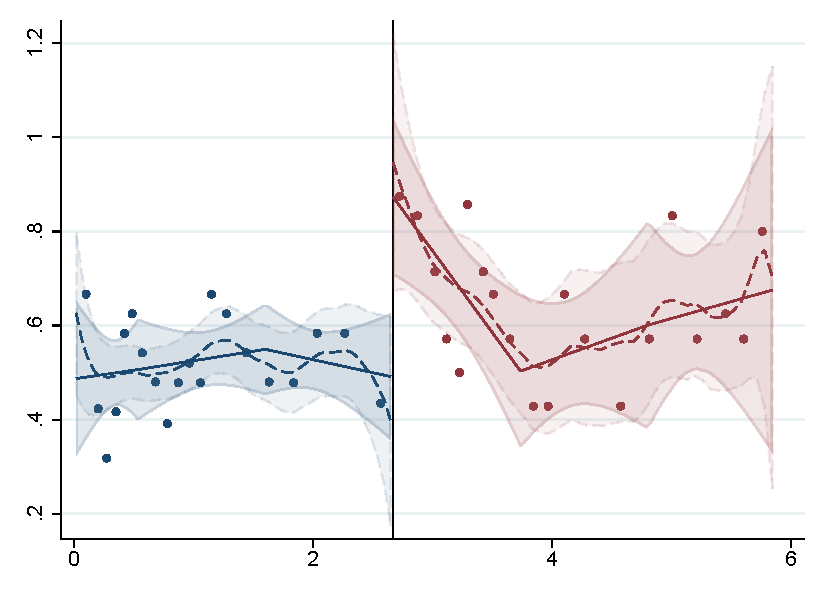
\includegraphics[width=\textwidth]{Figuras/rdplot_conflicto_arreglado_tenure_2.pdf}
    \end{subfigure}
    \begin{subfigure}{0.31\textwidth}
\caption{Daily wage}
        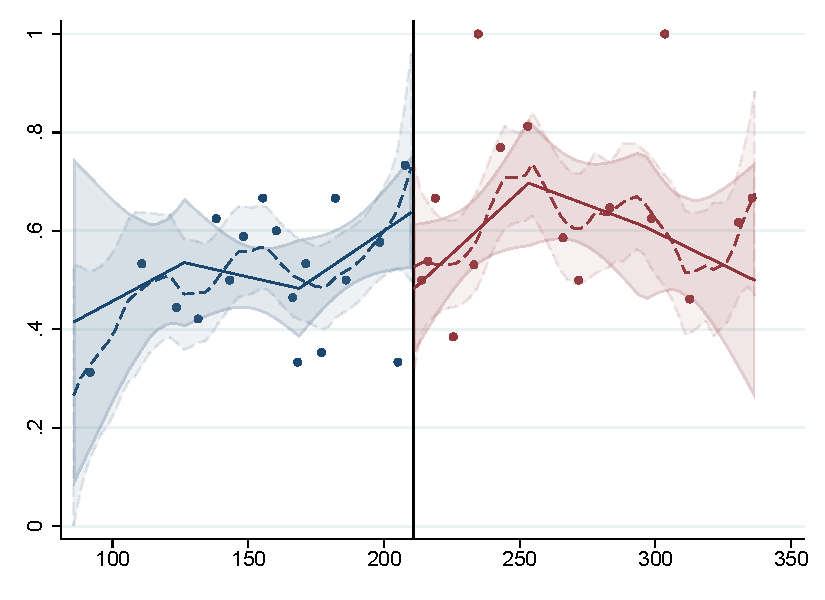
\includegraphics[width=\textwidth]{Figuras/rdplot_conflicto_arreglado_dw_2.pdf}
    \end{subfigure}        
    \begin{subfigure}{0.31\textwidth}
\caption{Tenure \& Daily wage}
        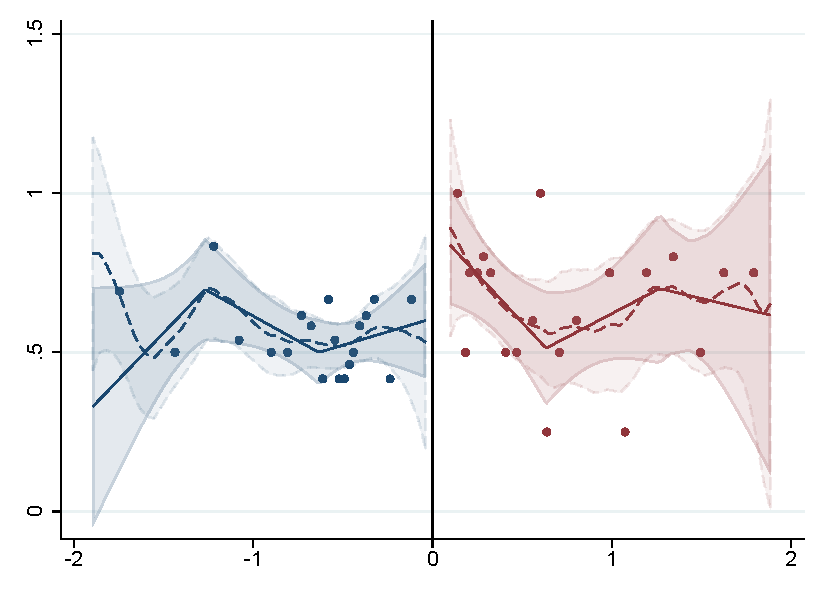
\includegraphics[width=\textwidth]{Figuras/rdplot_conflicto_arreglado_2_4_2.pdf}
    \end{subfigure}
  \end{center}
  
    \scriptsize Regression discontinuity plots using 1) local polynomial smoothing 2) B-splines.
%\textit{Scripts: }  \texttt{plot\_rd.do}
\end{figure}



%__________________________________________________________________________
%__________________________________________________________________________
%__________________________________________________________________________
%__________________________________________________________________________

\clearpage

\begin{figure}[H]
     \caption{RD plots (Calculator + letter treatment) - Effect on solved conflict}
    \label{rd_t3}
\begin{center}
\begin{subfigure}{0.31\textwidth}

\caption{Tenure}
        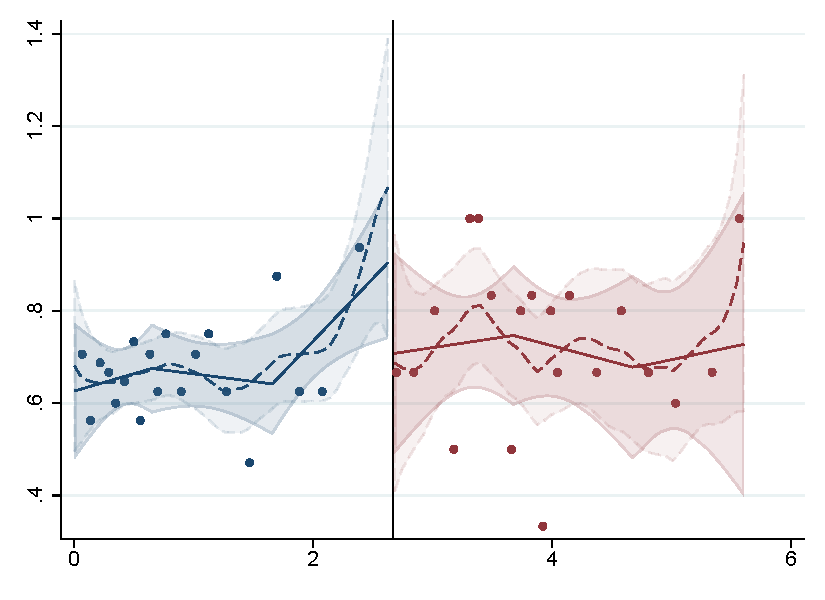
\includegraphics[width=\textwidth]{Figuras/rdplot_conflicto_arreglado_tenure_3.pdf}
    \end{subfigure}
    \begin{subfigure}{0.31\textwidth}
\caption{Daily wage}
        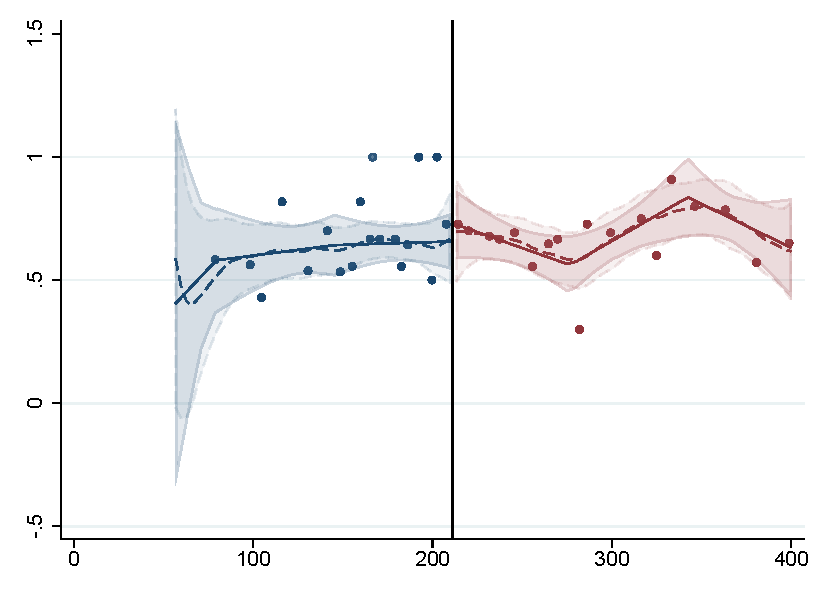
\includegraphics[width=\textwidth]{Figuras/rdplot_conflicto_arreglado_dw_3.pdf}
    \end{subfigure}        
    \begin{subfigure}{0.31\textwidth}
\caption{Tenure \& Daily wage}
        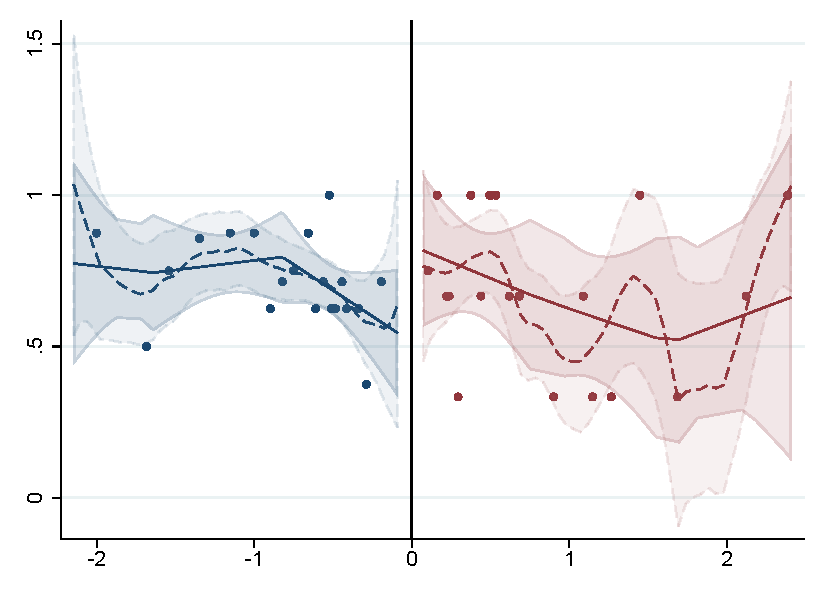
\includegraphics[width=\textwidth]{Figuras/rdplot_conflicto_arreglado_2_4_3.pdf}
    \end{subfigure}
  \end{center}
  
    \scriptsize Regression discontinuity plots using 1) local polynomial smoothing 2) B-splines.
%\textit{Scripts: }  \texttt{plot\_rd.do}
\end{figure}

\clearpage

\begin{figure}[H]
     \caption{RD plots (Calculator + letter treatment) - Effect on talking to a lawyer}
    \label{rd_t3}
\begin{center}
\begin{subfigure}{0.31\textwidth}

\caption{Tenure}
        \includegraphics[width=\textwidth]{Figuras/rdplot__tenure_3.pdf}
    \end{subfigure}
    \begin{subfigure}{0.31\textwidth}
\caption{Daily wage}
        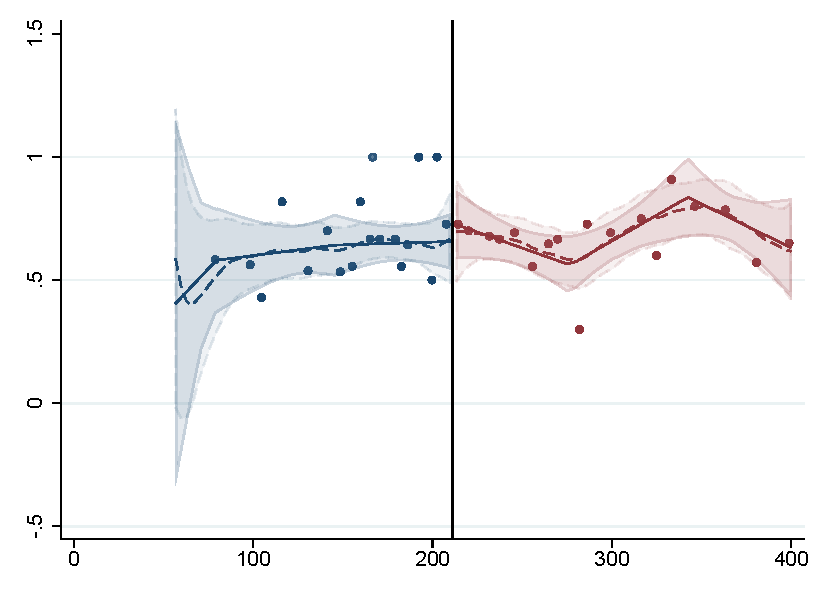
\includegraphics[width=\textwidth]{Figuras/rdplot_conflicto_arreglado_dw_3.pdf}
    \end{subfigure}        
    \begin{subfigure}{0.31\textwidth}
\caption{Tenure \& Daily wage}
        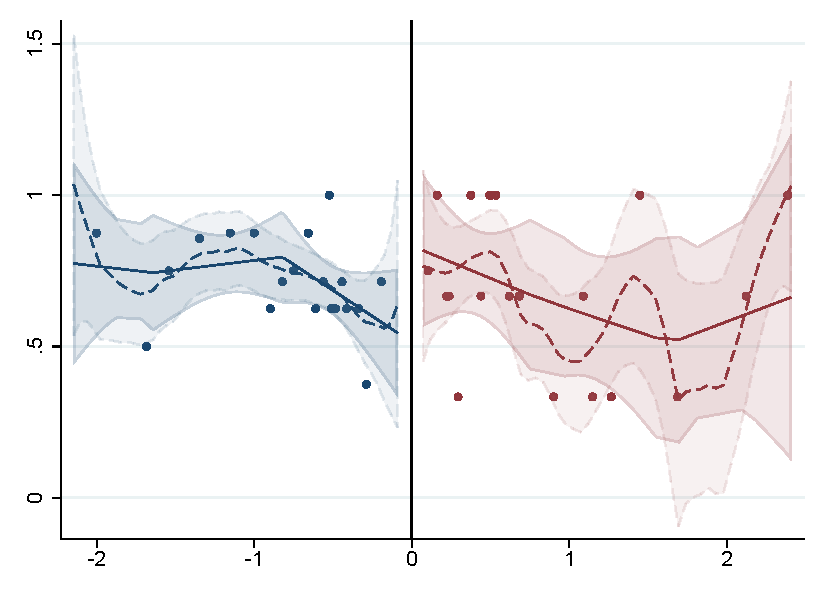
\includegraphics[width=\textwidth]{Figuras/rdplot_conflicto_arreglado_2_4_3.pdf}
    \end{subfigure}
  \end{center}
  
    \scriptsize Regression discontinuity plots using 1) local polynomial smoothing 2) B-splines.
%\textit{Scripts: }  \texttt{plot\_rd.do}
\end{figure}


%__________________________________________________________________________
%__________________________________________________________________________
%__________________________________________________________________________
%__________________________________________________________________________






\newpage
%  \documentclass[oneside,11pt]{article}

% \input{preamble.tex}
% %%% HELPER CODE FOR DEALING WITH EXTERNAL REFERENCES
% \usepackage{xr}
% \makeatletter
% \newcommand*{\addFileDependency}[1]{
%   \typeout{(#1)}
%   \@addtofilelist{#1}
%   \IfFileExists{#1}{}{\typeout{No file #1.}}
% }
% \makeatother


% \newcommand*{\myexternaldocument}[1]{
%     \externaldocument{#1}
%     \addFileDependency{#1.tex}
%     \addFileDependency{#1.aux}
% }

% %\myexternaldocument{OA}

% %%%%%%%%%%%%%%%%%%%%%%%%%%%%%%%% DOCUMENT
% \begin{document}

%%%%%%%%%%%%%%%%%%%%%%%%%%%%%%%%%%%%%%%%%%%%%%%

% APPENDIX 
\setcounter{table}{0}
\setcounter{figure}{0}
\setcounter{section}{0}
\pagenumbering{gobble}


\begin{center}
	\LARGE Bargaining with (more) common priors in the field \\[0.5em]
	\Large{Appendix $-$ For Online Publication} \\[1em]
	\large \author{Joyce Sadka \and Enrique Seira  \and Christopher Woodruff}
\end{center}

\appendix
\pagenumbering{arabic}
\renewcommand\thefigure{OA-\arabic{figure}}
\renewcommand\thetable{OA-\arabic{table}}
\renewcommand*{\thepage}{OA - \arabic{page}}
\renewcommand\thesection{Appendix \Alph{section}.}
\renewcommand\thesubsection{\Alph{section}.\arabic{subsection}}

%\renewcommand{\cftparskip}{0em} % NOT NEEDED
\renewcommand\cftsecdotsep{\cftdotsep}
\renewcommand\cftsubsecdotsep{\cftnodots}
\renewcommand{\cftsecnumwidth}{6em}
 \renewcommand{\cftpnumalign}{r}
%\renewcommand{\cftsecleader}{\normalfont\cftdotfill{\cftsecdotsep}}


\renewcommand{\cftsecleader}{\cftdotfill{\cftsecdotsep}\hspace{1.8em}}
%\renewcommand{\cftsecpagefont}{20em}
%\renewcommand{\cftfignumwidth}{6em}
%\renewcommand{\cfttabnumwidth}{3.3em}

%\tableofcontents
\etocdepthtag.toc{mtappendix}
\etocsettagdepth{mtchapter}{none}
\etocsettagdepth{mtappendix}{subsection}

\setstretch{0.9}
%\renewcommand\contentsname{} % the empty name

\begingroup
\let\clearpage\relax
%\vspace{-1.5em} % the removed space. Set as appropriate
\tableofcontents
\endgroup


\newpage

\section{ -Balance in covariates}
\vspace{.2in}

\begin{figure}[H]
     \caption{RD plots (Calculator treatment; running variable : Tenure)}
    \label{rd_covs_tenure_t2}
\begin{center}
\begin{subfigure}{0.31\textwidth}
\caption{Anger}
        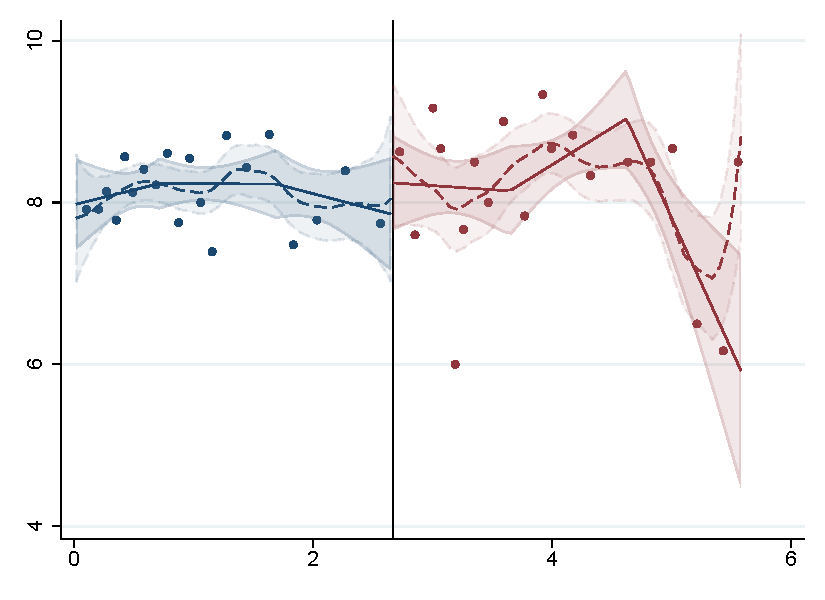
\includegraphics[width=\textwidth]{Figuras/rdplot_nivel_de_felicidad_tenure_2.pdf}
    \end{subfigure}
    \begin{subfigure}{0.31\textwidth}
\caption{More than High-School}
        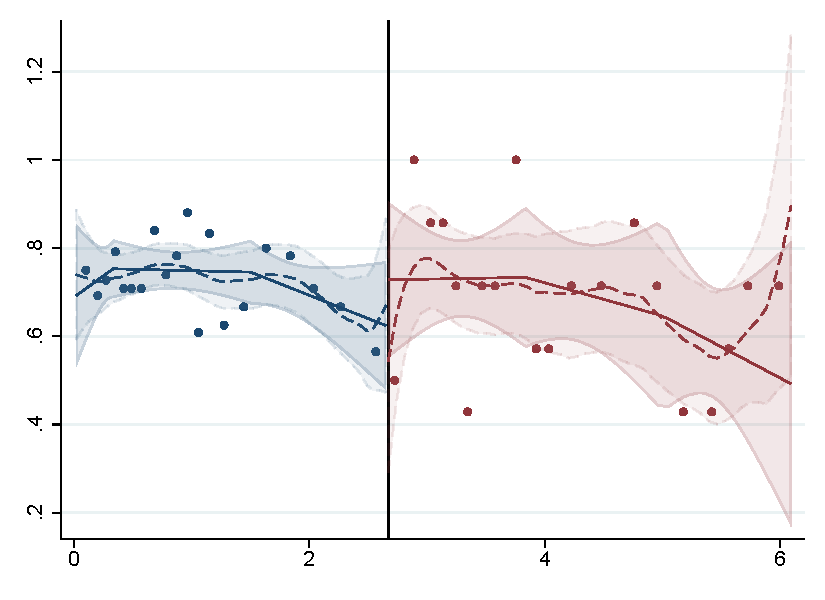
\includegraphics[width=\textwidth]{Figuras/rdplot_high_school_tenure_2.pdf}
    \end{subfigure}
\begin{subfigure}{0.31\textwidth}
\caption{Recruitment}
        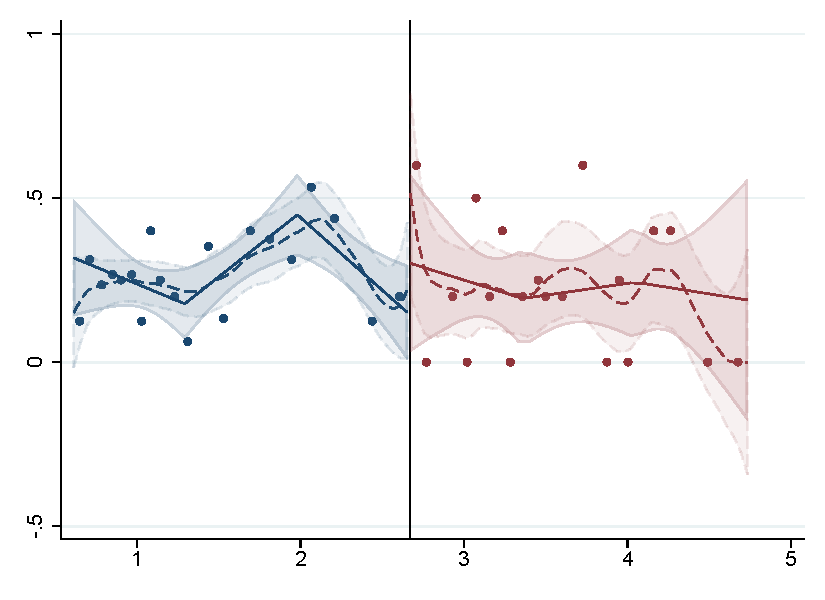
\includegraphics[width=\textwidth]{Figuras/rdplot_reclutamiento_tenure_2.pdf}
    \end{subfigure}
    \begin{subfigure}{0.31\textwidth}
\caption{At will worker}
        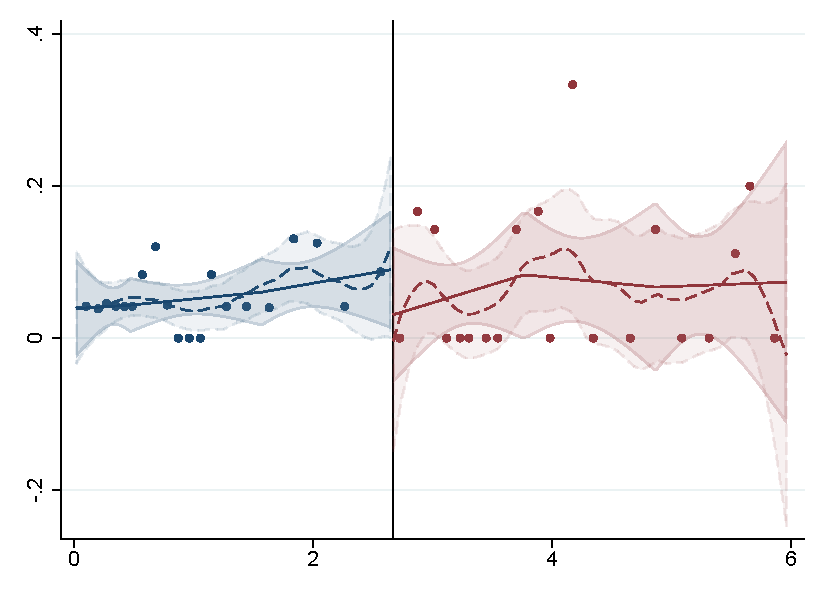
\includegraphics[width=\textwidth]{Figuras/rdplot_dummy_confianza_tenure_2.pdf}
    \end{subfigure}        
    \begin{subfigure}{0.31\textwidth}
\caption{Weekly hours}
        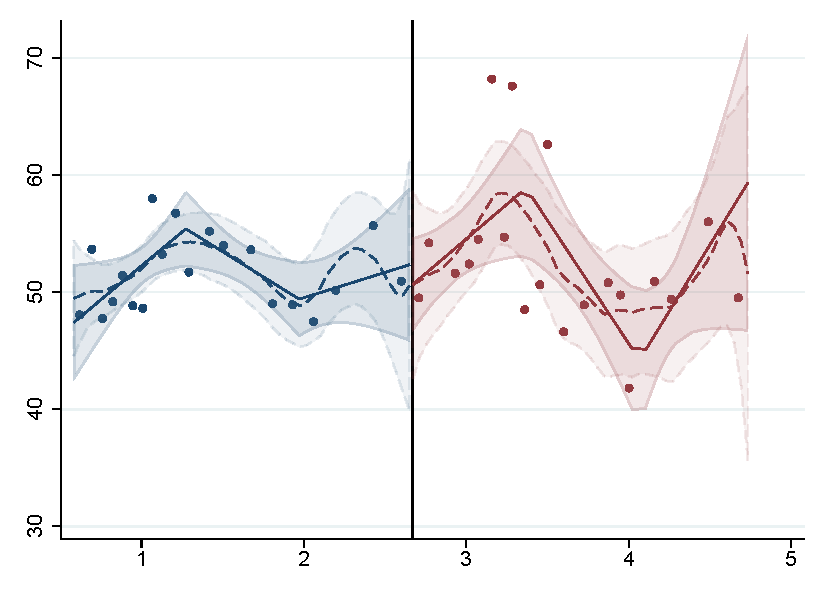
\includegraphics[width=\textwidth]{Figuras/rdplot_horas_sem_tenure_2.pdf}
    \end{subfigure}    
    \begin{subfigure}{0.31\textwidth}
\caption{Informal worker}
        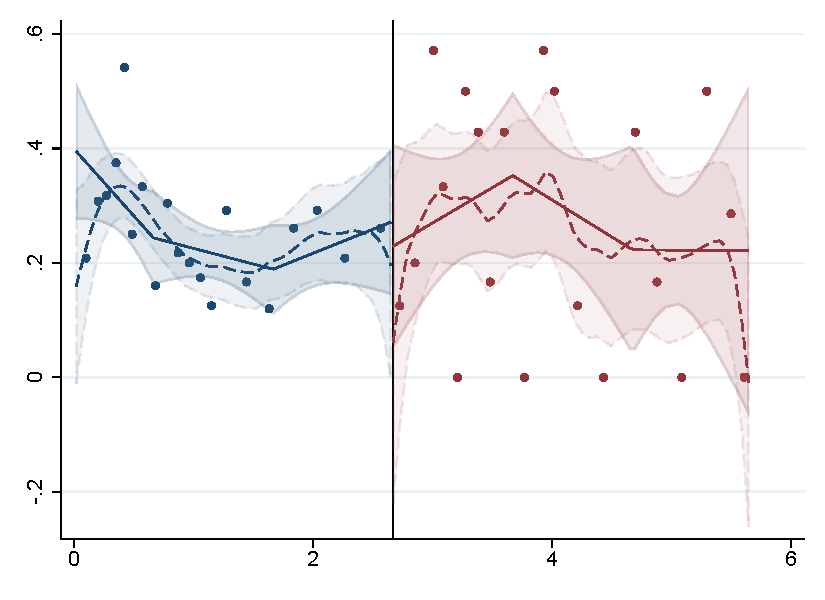
\includegraphics[width=\textwidth]{Figuras/rdplot_dummy_sarimssinfo_tenure_2.pdf}
    \end{subfigure}       
\begin{subfigure}{0.31\textwidth}
\caption{Legal entitlement}
        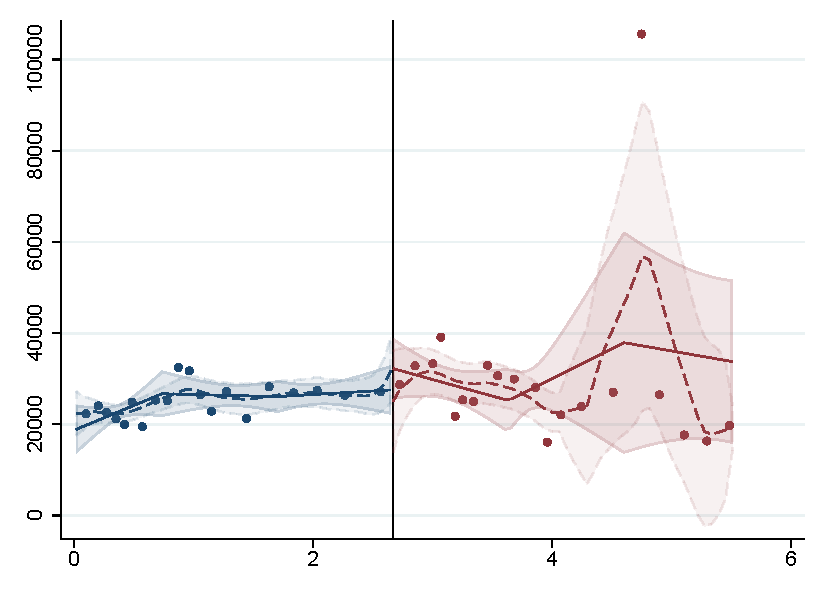
\includegraphics[width=\textwidth]{Figuras/rdplot_c_min_indem_tenure_2.pdf}
    \end{subfigure}
    \begin{subfigure}{0.31\textwidth}
\caption{Total entitlement}
        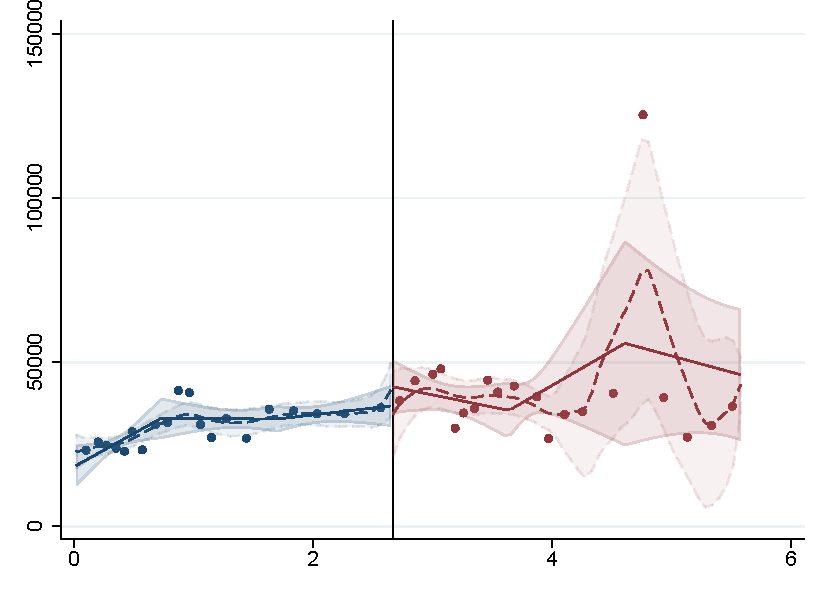
\includegraphics[width=\textwidth]{Figuras/rdplot_c_min_total_tenure_2.pdf}
    \end{subfigure}        
\begin{subfigure}{0.31\textwidth}
\caption{Woman}
        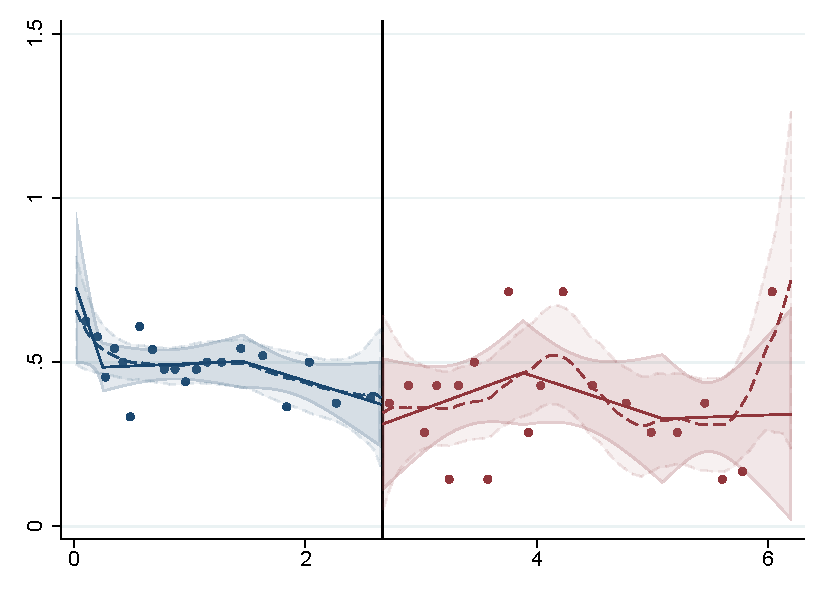
\includegraphics[width=\textwidth]{Figuras/rdplot_mujer_tenure_2.pdf}
    \end{subfigure}
  \end{center}
  
    \scriptsize Regression discontinuity plots using 1) local polynomial smoothing 2) B-splines. \textcolor{yellow}{Me falta ajustar cosas de inferencia cuando uso los splines.}
%\textit{Scripts: }  \texttt{plot\_rd\_covs.do}
\end{figure}




\begin{figure}[H]
     \caption{RD plots (Calculator treatment; running variable : Daily wage)}
    \label{rd_covs_dw_t2}
\begin{center}
\begin{subfigure}{0.31\textwidth}
\caption{Anger}
        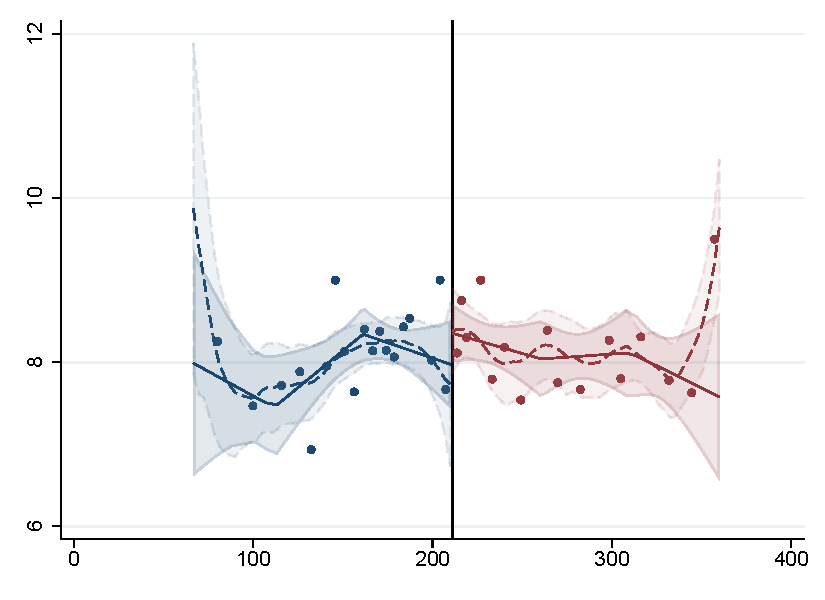
\includegraphics[width=\textwidth]{Figuras/rdplot_nivel_de_felicidad_dw_2.pdf}
    \end{subfigure}
    \begin{subfigure}{0.31\textwidth}
\caption{More than High-School}
        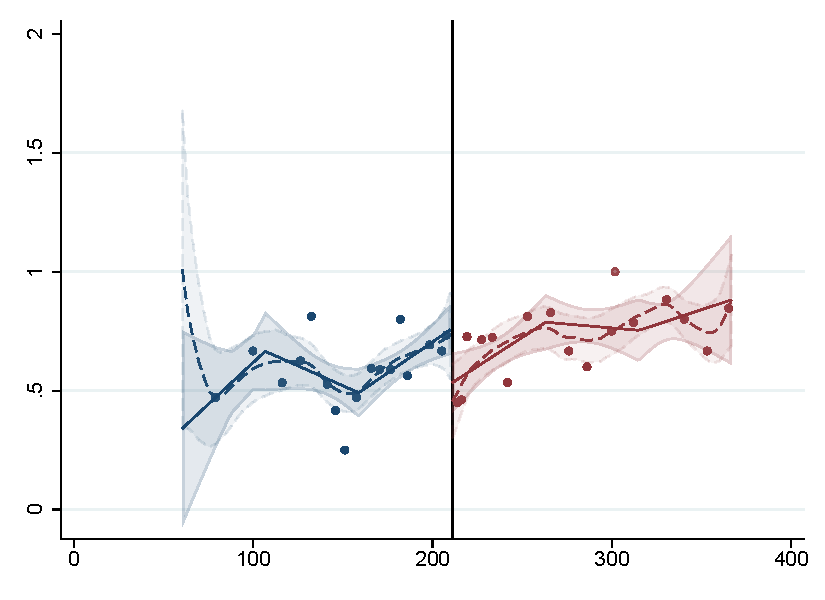
\includegraphics[width=\textwidth]{Figuras/rdplot_high_school_dw_2.pdf}
    \end{subfigure}
\begin{subfigure}{0.31\textwidth}
\caption{Recruitment}
        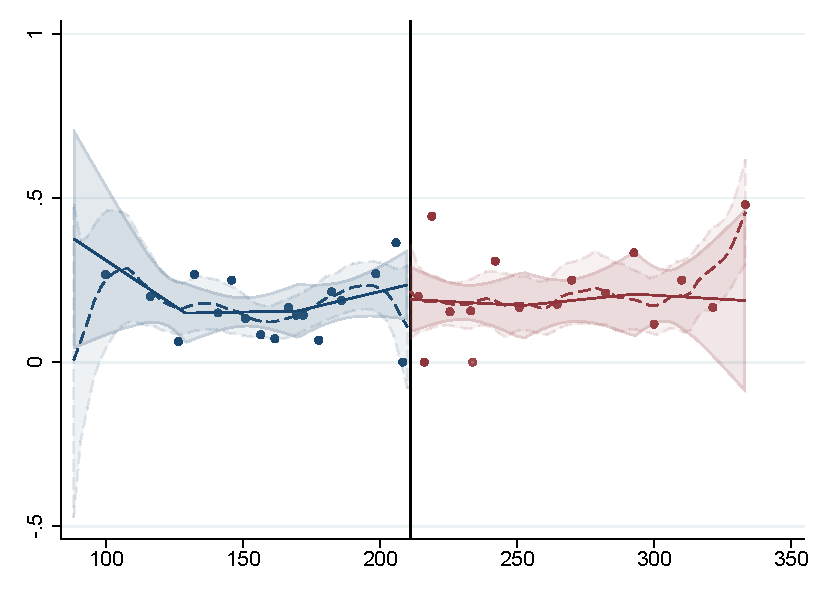
\includegraphics[width=\textwidth]{Figuras/rdplot_reclutamiento_dw_2.pdf}
    \end{subfigure}
    \begin{subfigure}{0.31\textwidth}
\caption{At will worker}
        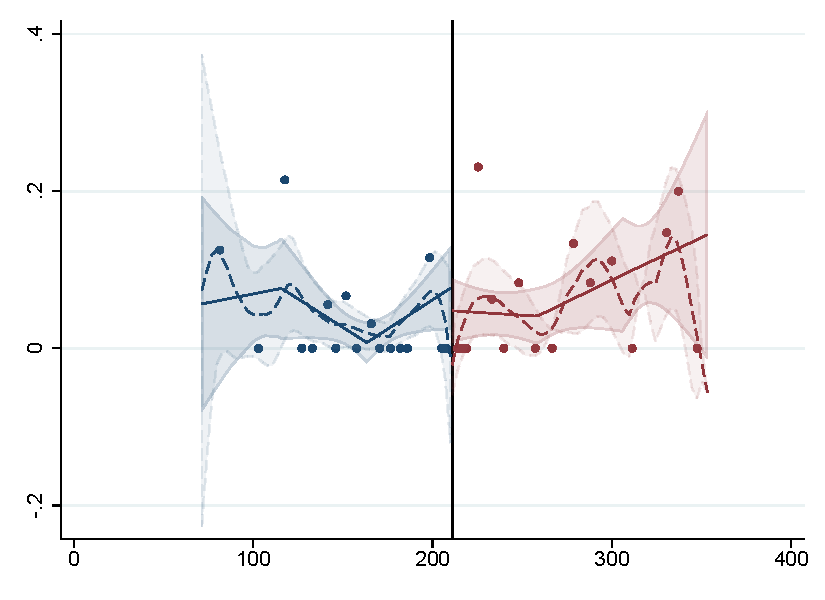
\includegraphics[width=\textwidth]{Figuras/rdplot_dummy_confianza_dw_2.pdf}
    \end{subfigure}        
    \begin{subfigure}{0.31\textwidth}
\caption{Weekly hours}
        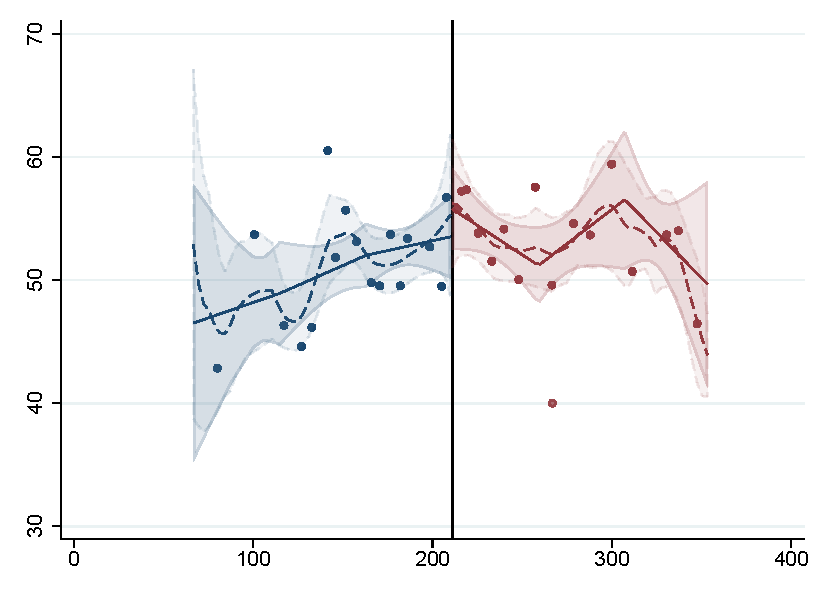
\includegraphics[width=\textwidth]{Figuras/rdplot_horas_sem_dw_2.pdf}
    \end{subfigure}    
    \begin{subfigure}{0.31\textwidth}
\caption{Informal worker}
        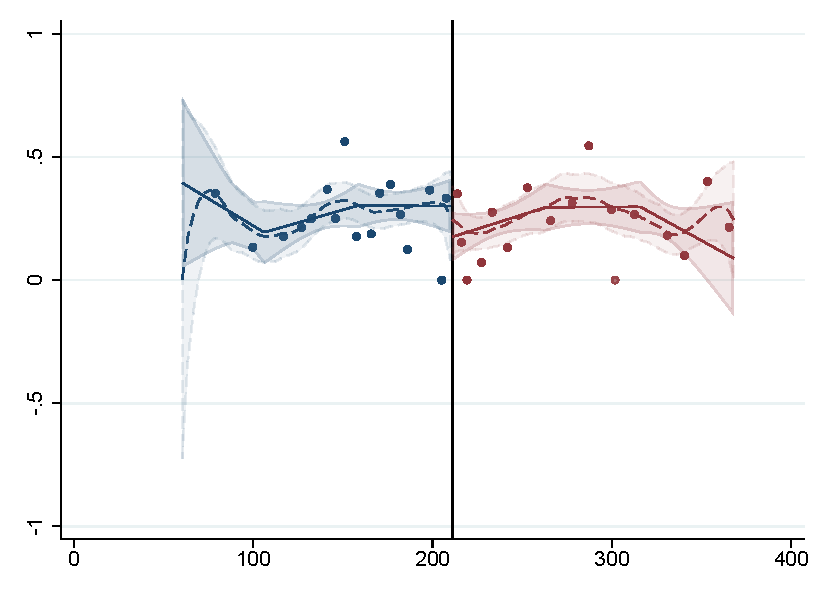
\includegraphics[width=\textwidth]{Figuras/rdplot_dummy_sarimssinfo_dw_2.pdf}
    \end{subfigure}       
\begin{subfigure}{0.31\textwidth}
\caption{Legal entitlement}
        \includegraphics[width=\textwidth]{Figuras/rdplot_c_min_indem_dw_2.pdf}
    \end{subfigure}
    \begin{subfigure}{0.31\textwidth}
\caption{Total entitlement}
        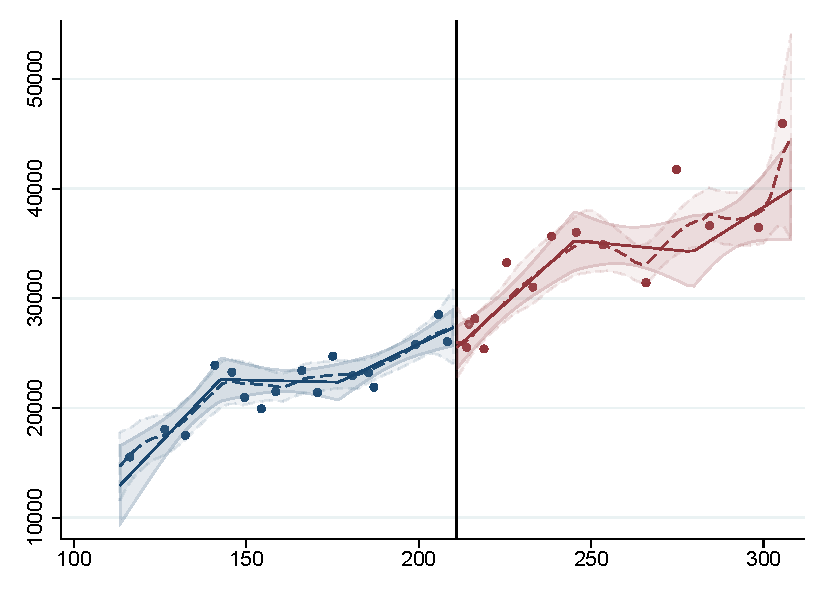
\includegraphics[width=\textwidth]{Figuras/rdplot_c_min_total_dw_2.pdf}
    \end{subfigure}        
\begin{subfigure}{0.31\textwidth}
\caption{Woman}
        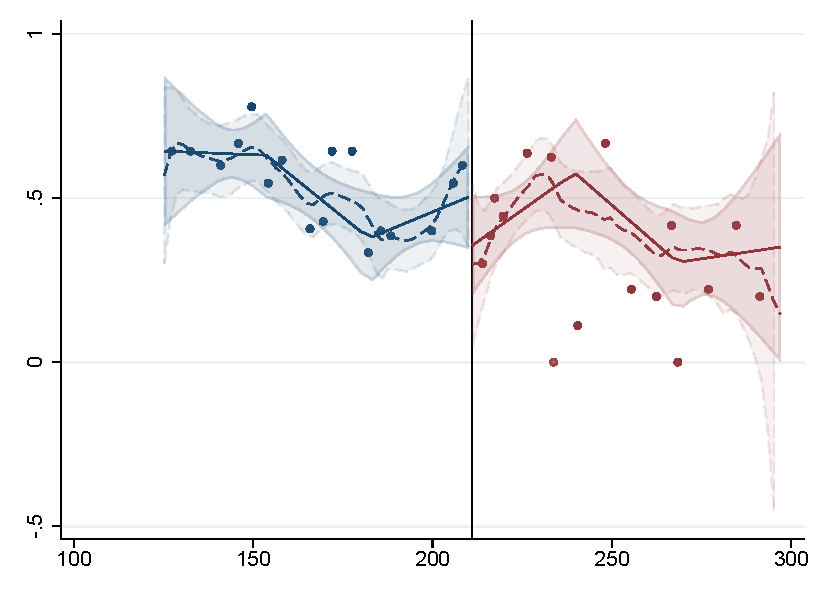
\includegraphics[width=\textwidth]{Figuras/rdplot_mujer_dw_2.pdf}
    \end{subfigure}
  \end{center}
  
    \scriptsize Regression discontinuity plots using 1) local polynomial smoothing 2) B-splines. \textcolor{yellow}{Me falta ajustar cosas de inferencia cuando uso los splines.}
%\textit{Scripts: }  \texttt{plot\_rd\_covs.do}
\end{figure}

\begin{figure}[H]
     \caption{RD plots (Calculator treatment; running variable : Tenure \& Daily wage)}
    \label{rd_covs_2_4_t2}
\begin{center}
\begin{subfigure}{0.31\textwidth}
\caption{Anger}
        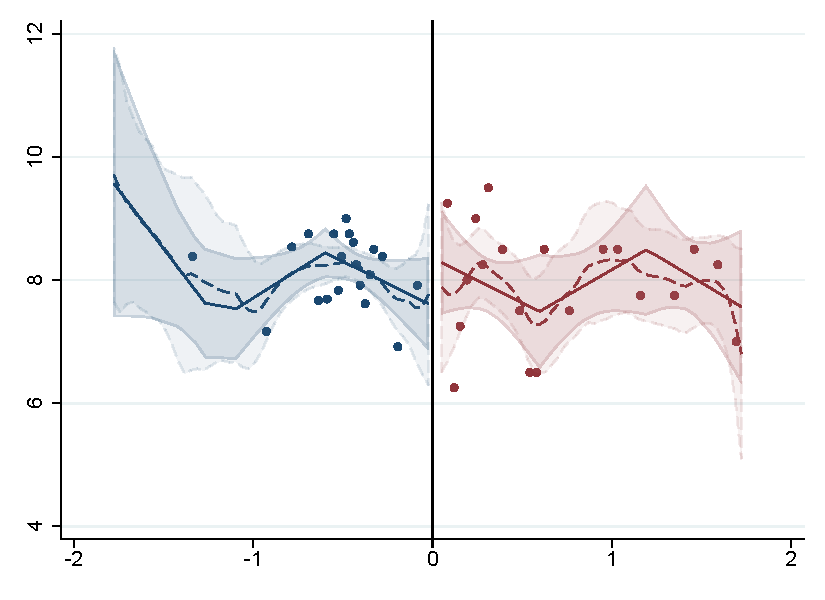
\includegraphics[width=\textwidth]{Figuras/rdplot_nivel_de_felicidad_2_4_2.pdf}
    \end{subfigure}
    \begin{subfigure}{0.31\textwidth}
\caption{More than High-School}
        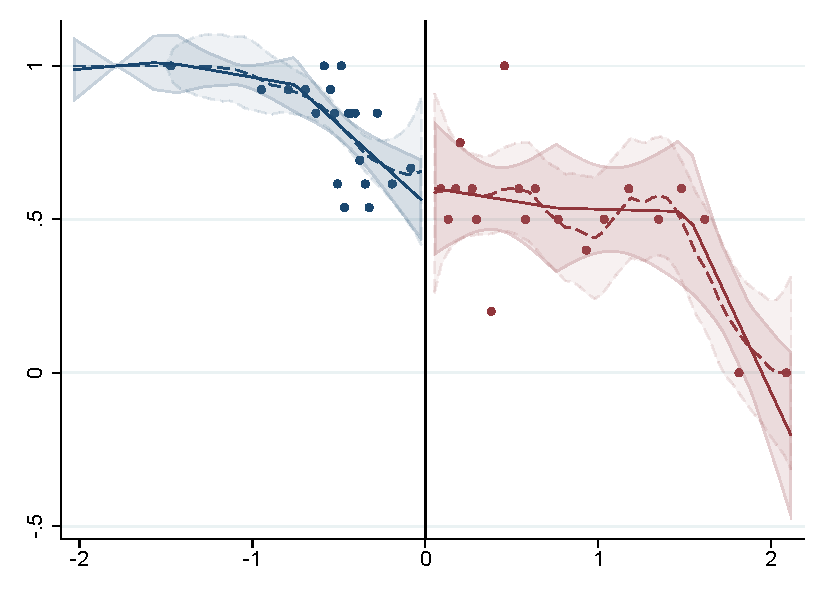
\includegraphics[width=\textwidth]{Figuras/rdplot_high_school_2_4_2.pdf}
    \end{subfigure}
\begin{subfigure}{0.31\textwidth}
\caption{Recruitment}
        \includegraphics[width=\textwidth]{Figuras/rdplot_reclutamiento_2_4_2.pdf}
    \end{subfigure}
    \begin{subfigure}{0.31\textwidth}
\caption{At will worker}
        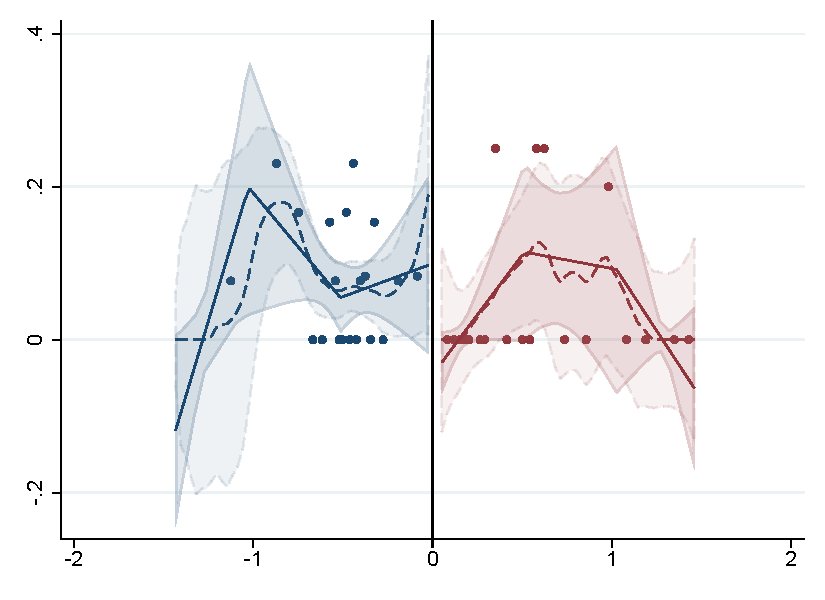
\includegraphics[width=\textwidth]{Figuras/rdplot_dummy_confianza_2_4_2.pdf}
    \end{subfigure}        
    \begin{subfigure}{0.31\textwidth}
\caption{Weekly hours}
        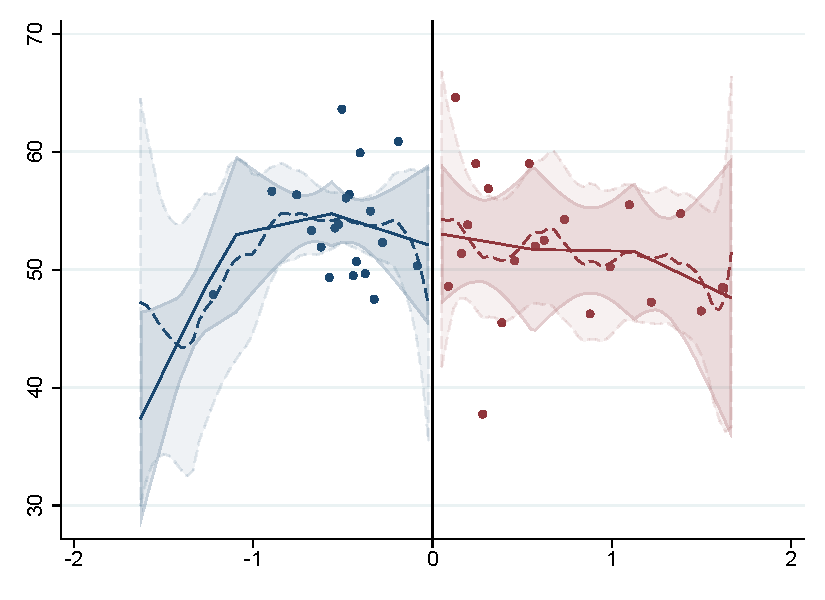
\includegraphics[width=\textwidth]{Figuras/rdplot_horas_sem_2_4_2.pdf}
    \end{subfigure}    
    \begin{subfigure}{0.31\textwidth}
\caption{Informal worker}
        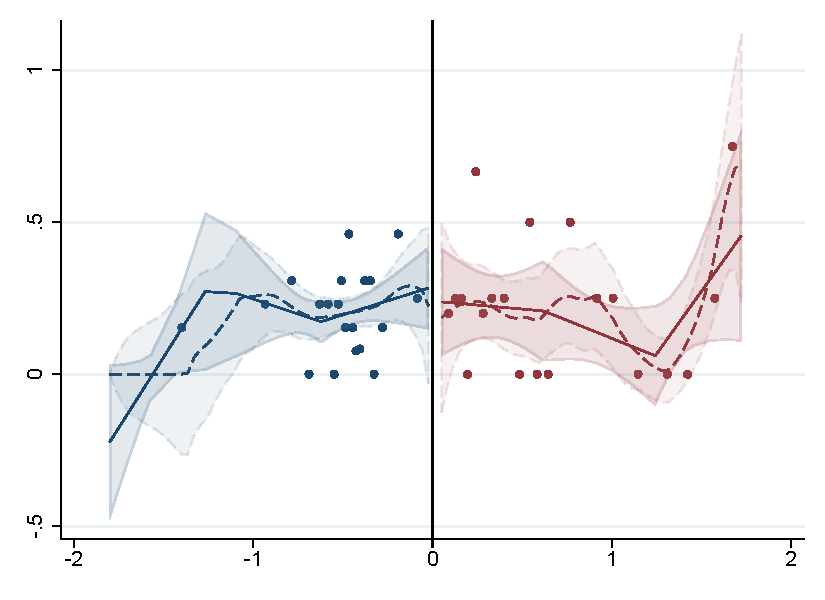
\includegraphics[width=\textwidth]{Figuras/rdplot_dummy_sarimssinfo_2_4_2.pdf}
    \end{subfigure}       
\begin{subfigure}{0.31\textwidth}
\caption{Legal entitlement}
        \includegraphics[width=\textwidth]{Figuras/rdplot_c_min_indem_2_4_2.pdf}
    \end{subfigure}
    \begin{subfigure}{0.31\textwidth}
\caption{Total entitlement}
        \includegraphics[width=\textwidth]{Figuras/rdplot_c_min_total_2_4_2.pdf}
    \end{subfigure}        
\begin{subfigure}{0.31\textwidth}
\caption{Woman}
        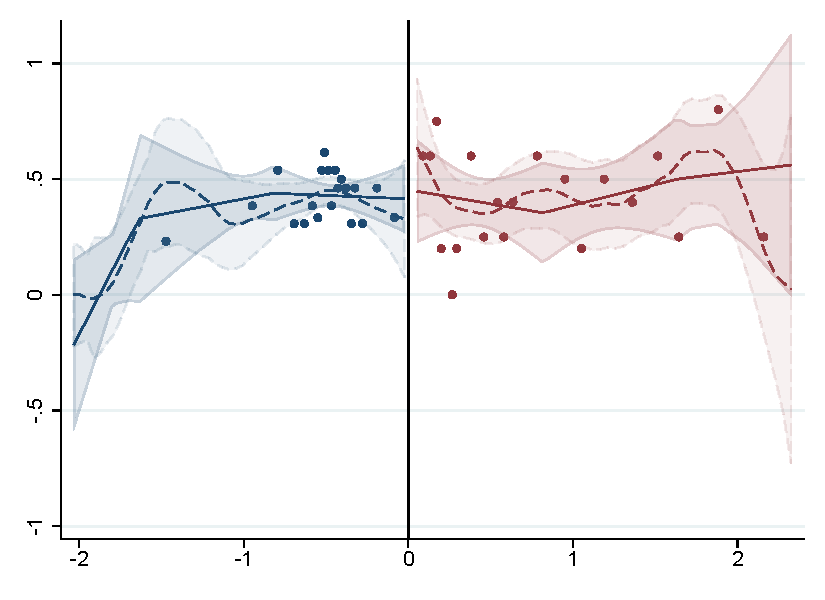
\includegraphics[width=\textwidth]{Figuras/rdplot_mujer_2_4_2.pdf}
    \end{subfigure}
  \end{center}
  
    \scriptsize Regression discontinuity plots using 1) local polynomial smoothing 2) B-splines. \textcolor{yellow}{Me falta ajustar cosas de inferencia cuando uso los splines.}
%\textit{Scripts: }  \texttt{plot\_rd\_covs.do}
\end{figure}


%__________________________________________________________________________
%__________________________________________________________________________
%__________________________________________________________________________
%__________________________________________________________________________

\section{ -Robustness : Validation and falsification of the RD design}
\vspace{.2in}


\begin{figure}[H]
     \caption{RD plots (Control)}
    \label{rd_t1}
\begin{center}
\begin{subfigure}{0.31\textwidth}

\caption{Tenure}
        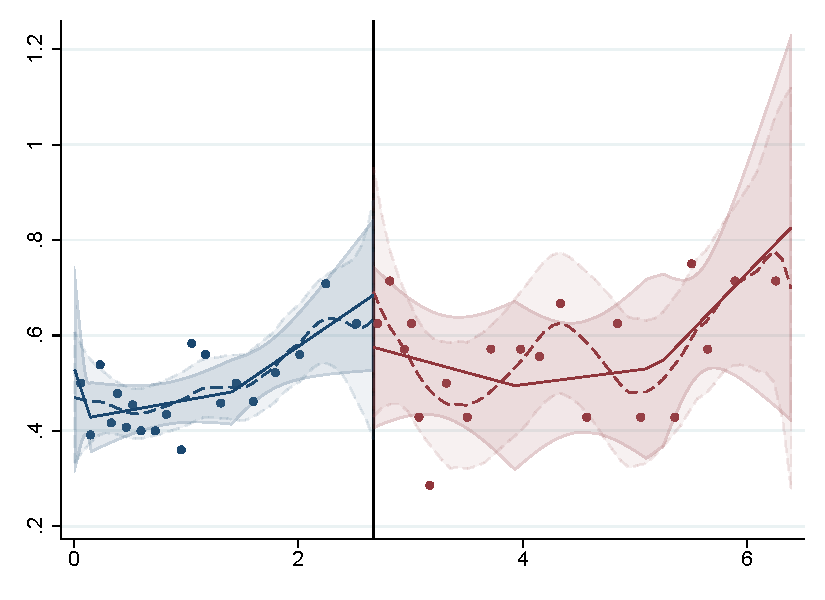
\includegraphics[width=\textwidth]{Figuras/rdplot_conflicto_arreglado_tenure_1.pdf}
    \end{subfigure}
    \begin{subfigure}{0.31\textwidth}
\caption{Daily wage}
        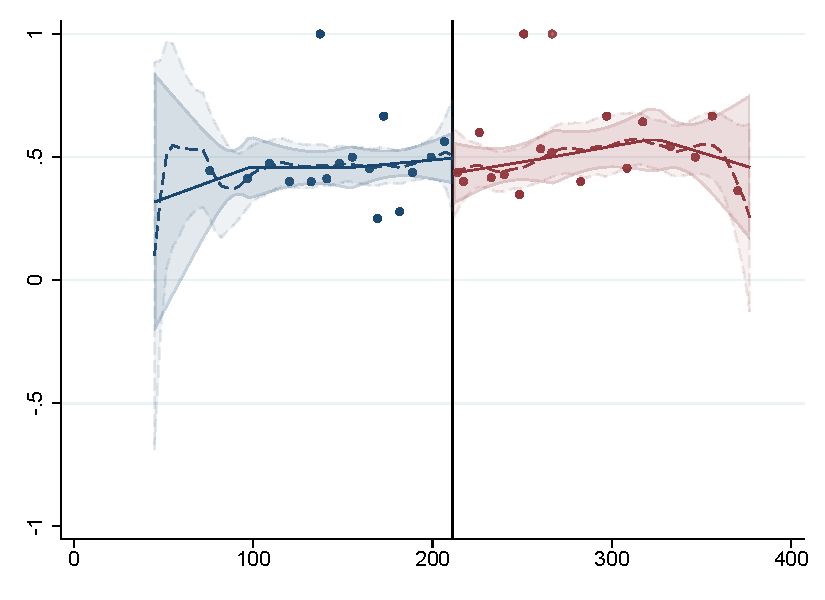
\includegraphics[width=\textwidth]{Figuras/rdplot_conflicto_arreglado_dw_1.pdf}
    \end{subfigure}        
    \begin{subfigure}{0.31\textwidth}
\caption{Tenure \& Daily wage}
        \includegraphics[width=\textwidth]{Figuras/rdplot_conflicto_arreglado_2_4_1.pdf}
    \end{subfigure}
  \end{center}
  
    \scriptsize Regression discontinuity plots using 1) local polynomial smoothing 2) B-splines. \textcolor{yellow}{Me falta ajustar cosas de inferencia cuando uso los splines.}
%\textit{Scripts: }  \texttt{plot\_rd\_control.do}
\end{figure}



%__________________________________________________________________________
%__________________________________________________________________________
%__________________________________________________________________________
%__________________________________________________________________________

\begin{figure}[H]
     \caption{Estimation for artificial cutoffs (Calculator treatment)}
    \label{placebo_cutoff_t2}
\begin{center}
\begin{subfigure}{0.475\textwidth}
\caption{Tenure}
        \includegraphics[width=\textwidth]{Figuras/placebo_cut_tenure_2.pdf}
    \end{subfigure}
    \begin{subfigure}{0.475\textwidth}
\caption{Daily wage}
        \includegraphics[width=\textwidth]{Figuras/placebo_cut_dw_2.pdf}
    \end{subfigure}
  \end{center}
  
    \scriptsize 
%\textit{Scripts: }  \texttt{placebo\_cutoff.do}
\end{figure}


\begin{figure}[H]
     \caption{Estimation for artificial cutoffs (Calculator + letter treatment)}
    \label{placebo_cutoff_t3}
\begin{center}
\begin{subfigure}{0.475\textwidth}
\caption{Tenure}
        \includegraphics[width=\textwidth]{Figuras/placebo_cut_tenure_3.pdf}
    \end{subfigure}
    \begin{subfigure}{0.475\textwidth}
\caption{Daily wage}
        \includegraphics[width=\textwidth]{Figuras/placebo_cut_dw_3.pdf}
    \end{subfigure}
  \end{center}
  
    \scriptsize 
%\textit{Scripts: }  \texttt{placebo\_cutoff.do}
\end{figure}



%__________________________________________________________________________
%__________________________________________________________________________
%__________________________________________________________________________
%__________________________________________________________________________

\begin{figure}[H]
     \caption{Donut-hole sensitivity (Calculator treatment)}
    \label{donut_hole_t2}
\begin{center}
\begin{subfigure}{0.475\textwidth}
\caption{Tenure}
        \includegraphics[width=\textwidth]{Figuras/donut_hole_tenure_2.pdf}
    \end{subfigure}
    \begin{subfigure}{0.475\textwidth}
\caption{Daily wage}
        \includegraphics[width=\textwidth]{Figuras/donut_hole_dw_2.pdf}
    \end{subfigure}
    \begin{subfigure}{0.475\textwidth}
\caption{Tenure \& Daily wage}
        \includegraphics[width=\textwidth]{Figuras/donut_hole_index_2.pdf}
    \end{subfigure}    
  \end{center}
  
    \scriptsize  If systematic manipulation of score values has occurred, it is natural to assume that the units closest to the cutoff are those most likely to have engaged in manipulation. The idea behind this approach is to exclude such units and then repeat the estimation and inference analysis using the remaining sample. This exercise is also useful to assess the sensitivity of the results to the unavoidable extrapolation involved in local polynomial estimation.
%\textit{Scripts: }  \texttt{donut\_hole.do}
\end{figure}


\begin{figure}[H]
     \caption{Donut-hole sensitivity (Calculator + letter treatment)}
    \label{donut_hole_t3}
\begin{center}
\begin{subfigure}{0.475\textwidth}
\caption{Tenure}
        \includegraphics[width=\textwidth]{Figuras/donut_hole_tenure_3.pdf}
    \end{subfigure}
    \begin{subfigure}{0.475\textwidth}
\caption{Daily wage}
        \includegraphics[width=\textwidth]{Figuras/donut_hole_dw_3.pdf}
    \end{subfigure}
    \begin{subfigure}{0.475\textwidth}
\caption{Tenure \& Daily wage}
        \includegraphics[width=\textwidth]{Figuras/donut_hole_index_3.pdf}
    \end{subfigure}    
  \end{center}
  
    \scriptsize  If systematic manipulation of score values has occurred, it is natural to assume that the units closest to the cutoff are those most likely to have engaged in manipulation. The idea behind this approach is to exclude such units and then repeat the estimation and inference analysis using the remaining sample. This exercise is also useful to assess the sensitivity of the results to the unavoidable extrapolation involved in local polynomial estimation.
%\textit{Scripts: }  \texttt{donut\_hole.do}
\end{figure}


%__________________________________________________________________________
%__________________________________________________________________________
%__________________________________________________________________________
%__________________________________________________________________________


\begin{figure}[H]
     \caption{Sensitivity to bandwidth choice (Calculator treatment)}
    \label{bwsensitivity_t2}
\begin{center}
\begin{subfigure}{0.475\textwidth}
\caption{Tenure}
        \includegraphics[width=\textwidth]{Figuras/bwsensitivity_tenure_2.pdf}
    \end{subfigure}
    \begin{subfigure}{0.475\textwidth}
\caption{Daily wage}
        \includegraphics[width=\textwidth]{Figuras/bwsensitivity_dw_2.pdf}
    \end{subfigure}
    \begin{subfigure}{0.475\textwidth}
\caption{Tenure \& Daily wage}
        \includegraphics[width=\textwidth]{Figuras/bwsensitivity_index_2.pdf}
    \end{subfigure}    
  \end{center}
  
    \scriptsize  RD treatment effect using different bandwidths. The x-axis is the multiplier for the bandwidth.
%\textit{Scripts: }  \texttt{sensitivity\_bw\_choice.do}
\end{figure}


\begin{figure}[H]
     \caption{Sensitivity to bandwidth choice (Calculator + letter treatment)}
    \label{bwsensitivity_t3}
\begin{center}
\begin{subfigure}{0.475\textwidth}
\caption{Tenure}
        \includegraphics[width=\textwidth]{Figuras/bwsensitivity_tenure_3.pdf}
    \end{subfigure}
    \begin{subfigure}{0.475\textwidth}
\caption{Daily wage}
        \includegraphics[width=\textwidth]{Figuras/bwsensitivity_dw_3.pdf}
    \end{subfigure}
    \begin{subfigure}{0.475\textwidth}
\caption{Tenure \& Daily wage}
        \includegraphics[width=\textwidth]{Figuras/bwsensitivity_index_3.pdf}
    \end{subfigure}    
  \end{center}
  
    \scriptsize  RD treatment effect using different bandwidths. The x-axis is the multiplier for the bandwidth.
%\textit{Scripts: }  \texttt{sensitivity\_bw\_choice.do}
\end{figure}



\clearpage
\bibliographystyle{authordate1}
%\bibliographystyle{amsalpha}
%\bibliographystyle{AER}

\bibliography{References}


\end{document}

\end{document}
